\section{PageRank}
\label{sec:graph-pagerank}

把网页看成顶点，链接看成有向边。只沿链接行走时，棋子可能进入走不出来的区域，也可能来到没有出边的页面。给行走加入重新选择顶点的机会，可以用长期分布为页面排名。这种做法称为\term{PageRank}\scite{page1999pagerank}。

\subsection{PageRank方程}
\label{sec:graph-pagerank-equation}

\paragraph{有向图的转移矩阵}

有向图的弧只从尾端指向头端。计算顶点$i$的转移概率时，只读取从$i$出去的弧，按出弧权重的总和归一化。

若某个顶点没有出边，就没有权重可以归一化。设$\bm{s}$为给定的概率行，用它补上零出度顶点所在的行。补齐后的$\bm{P}$每行非负、和为一，是一个行随机矩阵。

\paragraph{平稳分布的存在}

有限行随机矩阵总有平稳分布。为说明这一点，取任意概率初态$\bm{\nu}^{(0)}$，把前$T$步的分布取平均，
\[
\bm{a}^{(T)}=\frac{1}{T}\sum_{t=0}^{T-1}\bm{\nu}^{(0)}\bm{P}^t.
\]
右乘$\bm{P}$将每个时刻推进一步，新平均覆盖第$1$到第$T$步。中间$T-1$项相同，首尾两项之差除以$T$趋于零，
\[
\bm{a}^{(T)}\bm{P}-\bm{a}^{(T)}
=\frac{\bm{\nu}^{(0)}\bm{P}^T-\bm{\nu}^{(0)}}{T}
\to\bm{0}.
\]
这些平均都是概率行，位于有限维的闭有界集合中。从中选出一个收敛子列，极限就是平稳分布。

\paragraph{不唯一和振荡}

存在平稳分布之后，还要问它是否唯一、迭代能否收敛到它。

两个互不相连的有向环各有一个平稳分布，初态的分配方式会影响极限。即使平稳解唯一，迭代也可能振荡——一个两点有向环的唯一平稳分布是$(1/2,1/2)$，但从一点出发，分布在两个顶点之间永远交替。

\paragraph{重启机制}

为了同时解决不唯一和振荡，在每一步独立决定是否重启。以概率$\alpha\in(0,1)$按$\bm{s}$选择新位置，以概率$1-\alpha$按补齐后的$\bm{P}$转移。重启这一支不依赖当前位置，总使用同一份$\bm{s}$。

如果当前分布为$\bm{p}$，两支分别向下一步贡献$\alpha\bm{s}$和$(1-\alpha)\bm{p}\bm{P}$。要求下一步仍是$\bm{p}$，得到
\begin{equation}
\bm{p}=\alpha\bm{s}+(1-\alpha)\bm{p}\bm{P}.
\label{eq:graph-pagerank-fixed-point}
\end{equation}

这个方程还有另一种理解方式。先按$\bm{s}$选起点，每到一个位置，以概率$\alpha$结束，否则按$\bm{P}$再走一步。绕过前$t$次结束机会才在第$t+1$次结束，行走恰好走了$t$步，概率为$\alpha(1-\alpha)^t$。终点分布按步数加权求和，得
\begin{equation}
\bm{p}=\alpha\sum_{t=0}^{\infty}(1-\alpha)^t\bm{s}\bm{P}^t.
\label{eq:graph-pagerank-series}
\end{equation}
第零项对应立即结束的$\alpha\bm{s}$。把其余各项整体前移一个步数，提出公因子$(1-\alpha)$和一次$\bm{P}$，恰好得到$(1-\alpha)\bm{p}\bm{P}$。两部分相加满足式~\eqref{eq:graph-pagerank-fixed-point}。

\paragraph{唯一性与收敛性}

对任意两份概率差$\bm{z}$，一步转移不会放大$\ell^1$距离：逐列取绝对值并利用行和为一，$\lVert\bm{z}\bm{P}\rVert_1\le\lVert\bm{z}\rVert_1$。式~\eqref{eq:graph-pagerank-fixed-point}右端的更新映射$F$满足
\begin{equation}
\lVert F(\bm{x})-F(\bm{y})\rVert_1
\le(1-\alpha)\lVert\bm{x}-\bm{y}\rVert_1.
\label{eq:graph-pagerank-contraction}
\end{equation}
这是因为两个输入共享同一份重启$\alpha\bm{s}$，差值只出现在$1-\alpha$比例的转移部分。

若存在两个平稳解，更新后它们不变、距离不变，但收缩系数$1-\alpha<1$迫使距离为零。唯一性得证。从任意初态出发，第$t$轮与真解的距离每轮至少缩小为$1-\alpha$倍，因此迭代收敛。

\subsection{算法实现}
\label{sec:graph-pagerank-implementation}

输入为有向邻接表、概率行$\bm{s}$、重启概率$\alpha$和$\ell^1$误差容限$\varepsilon$。算法维护一份候选排名$\bm{p}^{(t)}$，从$\bm{p}^{(0)}=\bm{s}$开始。每一轮先沿实际出边传播概率，再加上重启部分。

\begin{algorithm}[PageRank迭代]
\label{alg:graph-pagerank-iteration}
输入：有向邻接表、概率行$\bm{s}$、重启概率$\alpha$、容许$\ell^1$误差$\varepsilon$。输出：近似排名$\bm{p}$。
\begin{enumerate}
  \item 令$\bm{p}^{(0)}=\bm{s}$。对零出度顶点记录标志。
  \item 每轮执行更新$\bm{p}^{(t+1)}=\alpha\bm{s}+(1-\alpha)\bm{p}^{(t)}\bm{P}$。实现时：先对每个正出度顶点$i$，把$(1-\alpha)p^{(t)}_i$按出边权重比例分给各头端。同时累计所有零出度顶点上的质量$q$，统一加回$q\bm{s}$。最后再加上重启项$\alpha\bm{s}$。
  \item 计算残差$\bm{r}=\bm{p}^{(t+1)}-\bm{p}^{(t)}$。若$\lVert\bm{r}\rVert_1\le\alpha\varepsilon$，返回$\bm{p}^{(t+1)}$。
\end{enumerate}
\end{algorithm}

每轮更新写成公式为
\begin{equation}
\bm{p}^{(t+1)}=\alpha\bm{s}+(1-\alpha)\bm{p}^{(t)}\bm{P}.
\label{eq:graph-pagerank-iteration}
\end{equation}

每轮先沿实际出边传播概率。对于零出度的顶点，只把它的分数加到悬挂质量$q$中。边扫描结束后，统一把$q\bm{s}$加到尚未乘$1-\alpha$的一步结果中。这等价于给每个悬挂点补上同一行$\bm{s}$，只需存一份重启分布。

考虑四个顶点及单位权弧$1\to2$、$2\to3$、$3\to1$、$3\to4$。顶点$4$没有出边。取$\bm{s}=(1,0,0,0)$、$\alpha=1/2$。每轮的重启部分给顶点$1$增加$1/2$的质量。

第一轮开始时全部质量在$1$，沿边部分的$1/2$送往$2$。第二轮将顶点$1$的质量减半后送到$2$，同时将$2$的质量减半后送到$3$，两点各得$1/4$。第三轮中，顶点$3$的$1/4$里有$1/2$沿边分出，分给$1,4$各$1/16$。这是顶点$4$首次收到质量。各轮结果为
\[
\begin{array}{c@{\qquad}c}
t&\bm{p}^{(t)}\\
1&(1/2,1/2,0,0)\\
2&(1/2,1/4,1/4,0)\\
3&(9/16,1/4,1/8,1/16)\\
4&(9/16,9/32,1/8,1/32)
\end{array}
\]
第四轮中，顶点$4$的旧质量$1/16$通过零出度填补分给顶点$1$，再乘沿边比例$1/2$，贡献$1/32$。同轮$3$也沿弧$3\to1$送来$1/32$。重启的$1/2$加上这两笔，$1$的新质量为$9/16$。图~\ref{fig:graph-pagerank-fourth-round}给出这一轮的各笔转移。

\begin{BookInlineFigure}
\centering
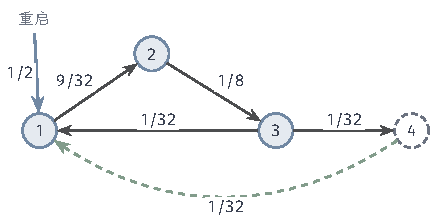
\includegraphics[width=73.459mm]{figures/03-graphs/05-matrices-and-spectra/tikz/walk-examples/pagerank-fourth-round.pdf}
\caption{四页算例在第四轮的质量分配，重启概率为$1/2$，重启集中到顶点$1$。深灰实线沿实际链接送出质量，虚线是零出度顶点$4$补齐后送出的份额。重启直接增加顶点$1$的质量。}
\label{fig:graph-pagerank-fourth-round}
\end{BookInlineFigure}

每轮所得各项非负，总和应为一，可据此检查传播、悬挂补偿和重启项是否漏加。

\subsection{算法分析}
\label{sec:graph-pagerank-cost}

由式~\eqref{eq:graph-pagerank-contraction}及两份概率行的$\ell^1$距离至多为$2$，第$t$轮的误差满足
\begin{equation}
\lVert\bm{p}^{(t)}-\bm{p}\rVert_1\le 2(1-\alpha)^t.
\label{eq:graph-pagerank-geometric-bound}
\end{equation}
要将上界压到$\varepsilon$，对$2(1-\alpha)^t\le\varepsilon$取对数，得到充分的迭代轮数
\[
t\ge \left\lceil\frac{\log(2/\varepsilon)}{-\log(1-\alpha)}\right\rceil.
\]
例如$\alpha=1/2$时，六轮可把上界压到$1/32$。当$\alpha$很小时，$-\log(1-\alpha)$与$\alpha$同阶，轮数约为$\alpha^{-1}\log(2/\varepsilon)$。

在运行中，真解$\bm{p}$未知，但可以计算候选$\bm{q}$再走一轮会变多少。记残差为$\bm{r}=F(\bm{q})-\bm{q}$。从$\bm{q}$到真解$\bm{p}$的距离，可以先走到$F(\bm{q})$再走到$F(\bm{p})=\bm{p}$。第一段距离是$\lVert\bm{r}\rVert_1$，第二段由收缩性控制，因此
\[
\lVert\bm{q}-\bm{p}\rVert_1
\le\lVert\bm{r}\rVert_1+(1-\alpha)\lVert\bm{q}-\bm{p}\rVert_1.
\]
移项得到
\begin{equation}
\lVert\bm{q}-\bm{p}\rVert_1\le\frac{\lVert\bm{r}\rVert_1}{\alpha}.
\label{eq:graph-pagerank-residual-bound}
\end{equation}
若残差范数不超过$\alpha\varepsilon$，当前候选的误差就不超过$\varepsilon$。

设图有$n$个顶点、$m$条弧。每轮传播扫描$m$条弧，初始化和悬挂补偿需$O(n)$。每轮时间和整个存储均为$O(n+m)$。

$\alpha$越大，一次行走越可能很快结束，终点分布越接近$\bm{s}$，迭代也越快收敛。较小的$\alpha$留下更多沿边传播的机会，但也让每轮保留更多旧误差。选择$\alpha$同时改变排名的含义和计算的速度。
